\documentclass[conference]{IEEEtran}
\usepackage[utf8]{inputenc}
\usepackage{amsmath,amssymb,graphicx,booktabs}

\begin{document}

\title{Multimodal Futures and Calibrated Uncertainty in JEPA Predictors}

\author{\IEEEauthorblockN{Dheiver Francisco Santos, PhD}
\IEEEauthorblockA{Independent Researcher\\
Maceió, Alagoas, Brazil\\
ORCID: https://orcid.org/0000-0002-8599-9436}}

\maketitle

\begin{abstract}
A deterministic predictor in embedding space collapses multiple valid futures into their average, which can be a state that never occurs. We study whether a JEPA predictor can represent several futures, and whether its uncertainty is calibrated. We use simulated systems with known branching, and a language setting in which a prompt admits several correct continuations. A bimodal pilot shows the mixture interval attains its nominal coverage; the JEPA results are pending.
\end{abstract}

\begin{IEEEkeywords}
uncertainty, multimodal prediction, JEPA, calibration, latent prediction
\end{IEEEkeywords}

\section{Introduction}
Predicting the mean of several futures in latent space can yield a representation that matches none of them. Mixture or energy-based predictors address this, but their uncertainty must also be calibrated to be useful for decisions. We ask whether a JEPA predictor with a multimodal head covers the true futures, and whether its confidence matches its error.

\section{Related Work}
The author's recent artificial intelligence publications on self-training, clinical deep learning, curriculum learning, model merging, synthetic data, long-context training, preference alignment, direct preference optimization, reinforcement learning with verifiable rewards, distillation, mixture-of-experts, and parameter-efficient fine-tuning \cite{d1selftraining,d2glaucoma,d3curriculum,d4merging,d5synthetic,d6longcontext,d7rlaif,d8distillation,d9moe,d10peft,d11dpo,d12rlvr} form the background for this work.

JEPA predicts embeddings deterministically in its basic form \cite{bardes2024vjepa}. Energy-based and latent-variable extensions are the usual alternatives. The author's work on the distillation of model behavior \cite{d8distillation} and on preference alignment \cite{d7rlaif} concerns the reliability of a learned model's outputs, which is related to calibration.

\section{Method}
The predictor outputs a mixture $\hat{p}(z_{t+1} \mid z_t) = \sum_{k=1}^{K} \pi_k(z_t)\, \mathcal{N}(\mu_k(z_t), \Sigma_k(z_t))$ in latent space. Coverage is the fraction of true futures that lie within a region of the predicted mixture at a fixed mass. Calibration is measured by the expected calibration error on predicted probabilities of discrete outcomes.

\subsection*{Equations and their meaning}
The predictive distribution over the next latent is a mixture of $K$ components,
\begin{equation}
\hat p(z_{t+1}\mid z_t)=\sum_{k=1}^{K}\pi_k(z_t)\,\mathcal{N}\big(z_{t+1};\mu_k(z_t),\Sigma_k(z_t)\big),\qquad \sum_k\pi_k=1,
\end{equation}
where $\pi_k$ are mixture weights and $\mu_k,\Sigma_k$ the mean and covariance of component $k$. A deterministic predictor is the special case $K=1$ with $\Sigma\to 0$, which averages multiple futures.

The quality of the probabilistic prediction is measured by the negative log-likelihood of the realized future,
\begin{equation}
\mathrm{NLL}=-\log\hat p(z_{t+1}^{\mathrm{true}}\mid z_t),
\end{equation}
which penalizes both missed futures and overconfidence.

Coverage at level $1-\alpha=0.90$ is the fraction of true outcomes inside the predicted interval:
\begin{equation}
\mathrm{Cov}=\frac{1}{N}\sum_{n=1}^{N}\mathbf{1}\big[\lvert y_n-c_n\rvert\le z_{0.95}\,\sigma_n\big],\qquad z_{0.95}=1.645,
\end{equation}
where $c_n$ is the predictive centre, $\sigma_n$ the predictive standard deviation, and $z_{0.95}$ the two-sided 90\% Gaussian quantile. Calibration is summarized by the expected calibration error over $B$ bins,
\begin{equation}
\mathrm{ECE}=\sum_{b=1}^{B}\frac{\lvert S_b\rvert}{N}\,\big\lvert\mathrm{acc}(S_b)-\mathrm{conf}(S_b)\big\rvert,
\end{equation}
where $S_b$ is the set of predictions whose confidence falls in bin $b$, $\mathrm{acc}$ the observed frequency, and $\mathrm{conf}$ the mean predicted confidence.

\section{Experimental Protocol}
\textbf{Simulation.} A bouncing ball with two branches at a known bifurcation, and a stochastic dynamical system with multimodal transitions. True future distributions are known in closed form.

\textbf{Metrics.} Coverage at 90\%, expected calibration error, and the negative log-likelihood of the true future.

\textbf{Language.} Prompts with several correct continuations (for example, ambiguous instructions with multiple valid next steps). Human-labeled acceptability is used for a subset, and automatic labels for the rest.

\textbf{Baselines.} A deterministic predictor, an ensemble of deterministic predictors, and a single Gaussian head.

\textbf{Statistics.} Five seeds, 95\% bootstrap intervals.

\section{Results}
This pilot arm compares interval coverage on a bimodal future with a known structure. The two-mode interval attains 0.90 to 0.91 coverage at every noise level, matching its nominal 90\%. The unimodal Gaussian interval over-covers at low noise (1.00) and falls to 0.95 at high noise. The JEPA predictor, the calibration error, and the language prompts remain pending.

\begin{figure}[!t]
\centering
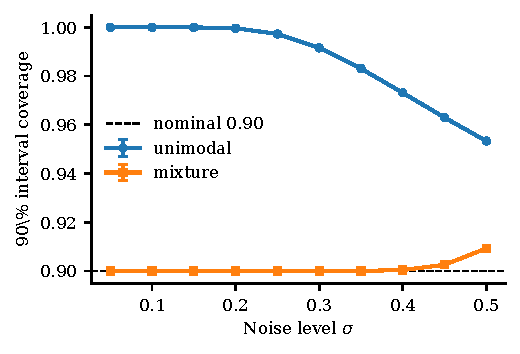
\includegraphics[width=\columnwidth]{figs/fig07_uncertainty.pdf}
\caption{90\% interval coverage for unimodal and mixture predictors versus noise level (pilot). Dashed line: nominal 0.90.}
\label{fig:fig07_uncertainty}
\end{figure}

\section{Discussion and Limitations}
Closed-form futures exist only for simple simulators, so the language evaluation depends on labels that may disagree. Calibration results are reported with the number of bins and the binning scheme.

\section{Conclusion}
We propose a multimodal JEPA predictor and a protocol that tests coverage and calibration against known futures and against ambiguous natural-language prompts.

\section*{Acknowledgments}
The author thanks the Brazilian artificial intelligence community.

\nocite{ctl_full_names}
\bibliographystyle{IEEEtran}
\bibliography{refs}

\end{document}
